\section{iClusterVB Implementation on Breast Cancer data}

In this section, we transition from working with simulation data to applying our
methodology to a more realistic dataset. 

Specifically, we utilize the Breast Cancer dataset obtained from Kaggle.
This dataset provides a practical context to evaluate the performance 
and applicability of the iClusterVB implementation in addressing real-world challenges.


There are no missing values in the dataset, and all features are numeric(except the target variable(M \& B)), which provide 
us convenient conditions for applying the iClusterVB method.

Before taking statistical testing, we did some data preprocessing. We encoded the target variable and split the data based on the 
target variable, got two subsets of data, one for M and one for B.  After checking the distributions of the two data sets,
we found there were heavy skewness and outliers in the data, therefore we make a simple logarithm transformation on the data
\footnote{In later practice, other transfomration can be used here, taking log-transfomration is only for convenience of demonstration
here}.

\subsection{Distribution Testing}
By normality testing, we found that most variables are not normally distributed,
only four variables are normally distributed, which are: \textit{area\_se, texture\_worst, concave points\_worst, symmetry\_worst}.

\begin{figure}[!h]
    \centering
    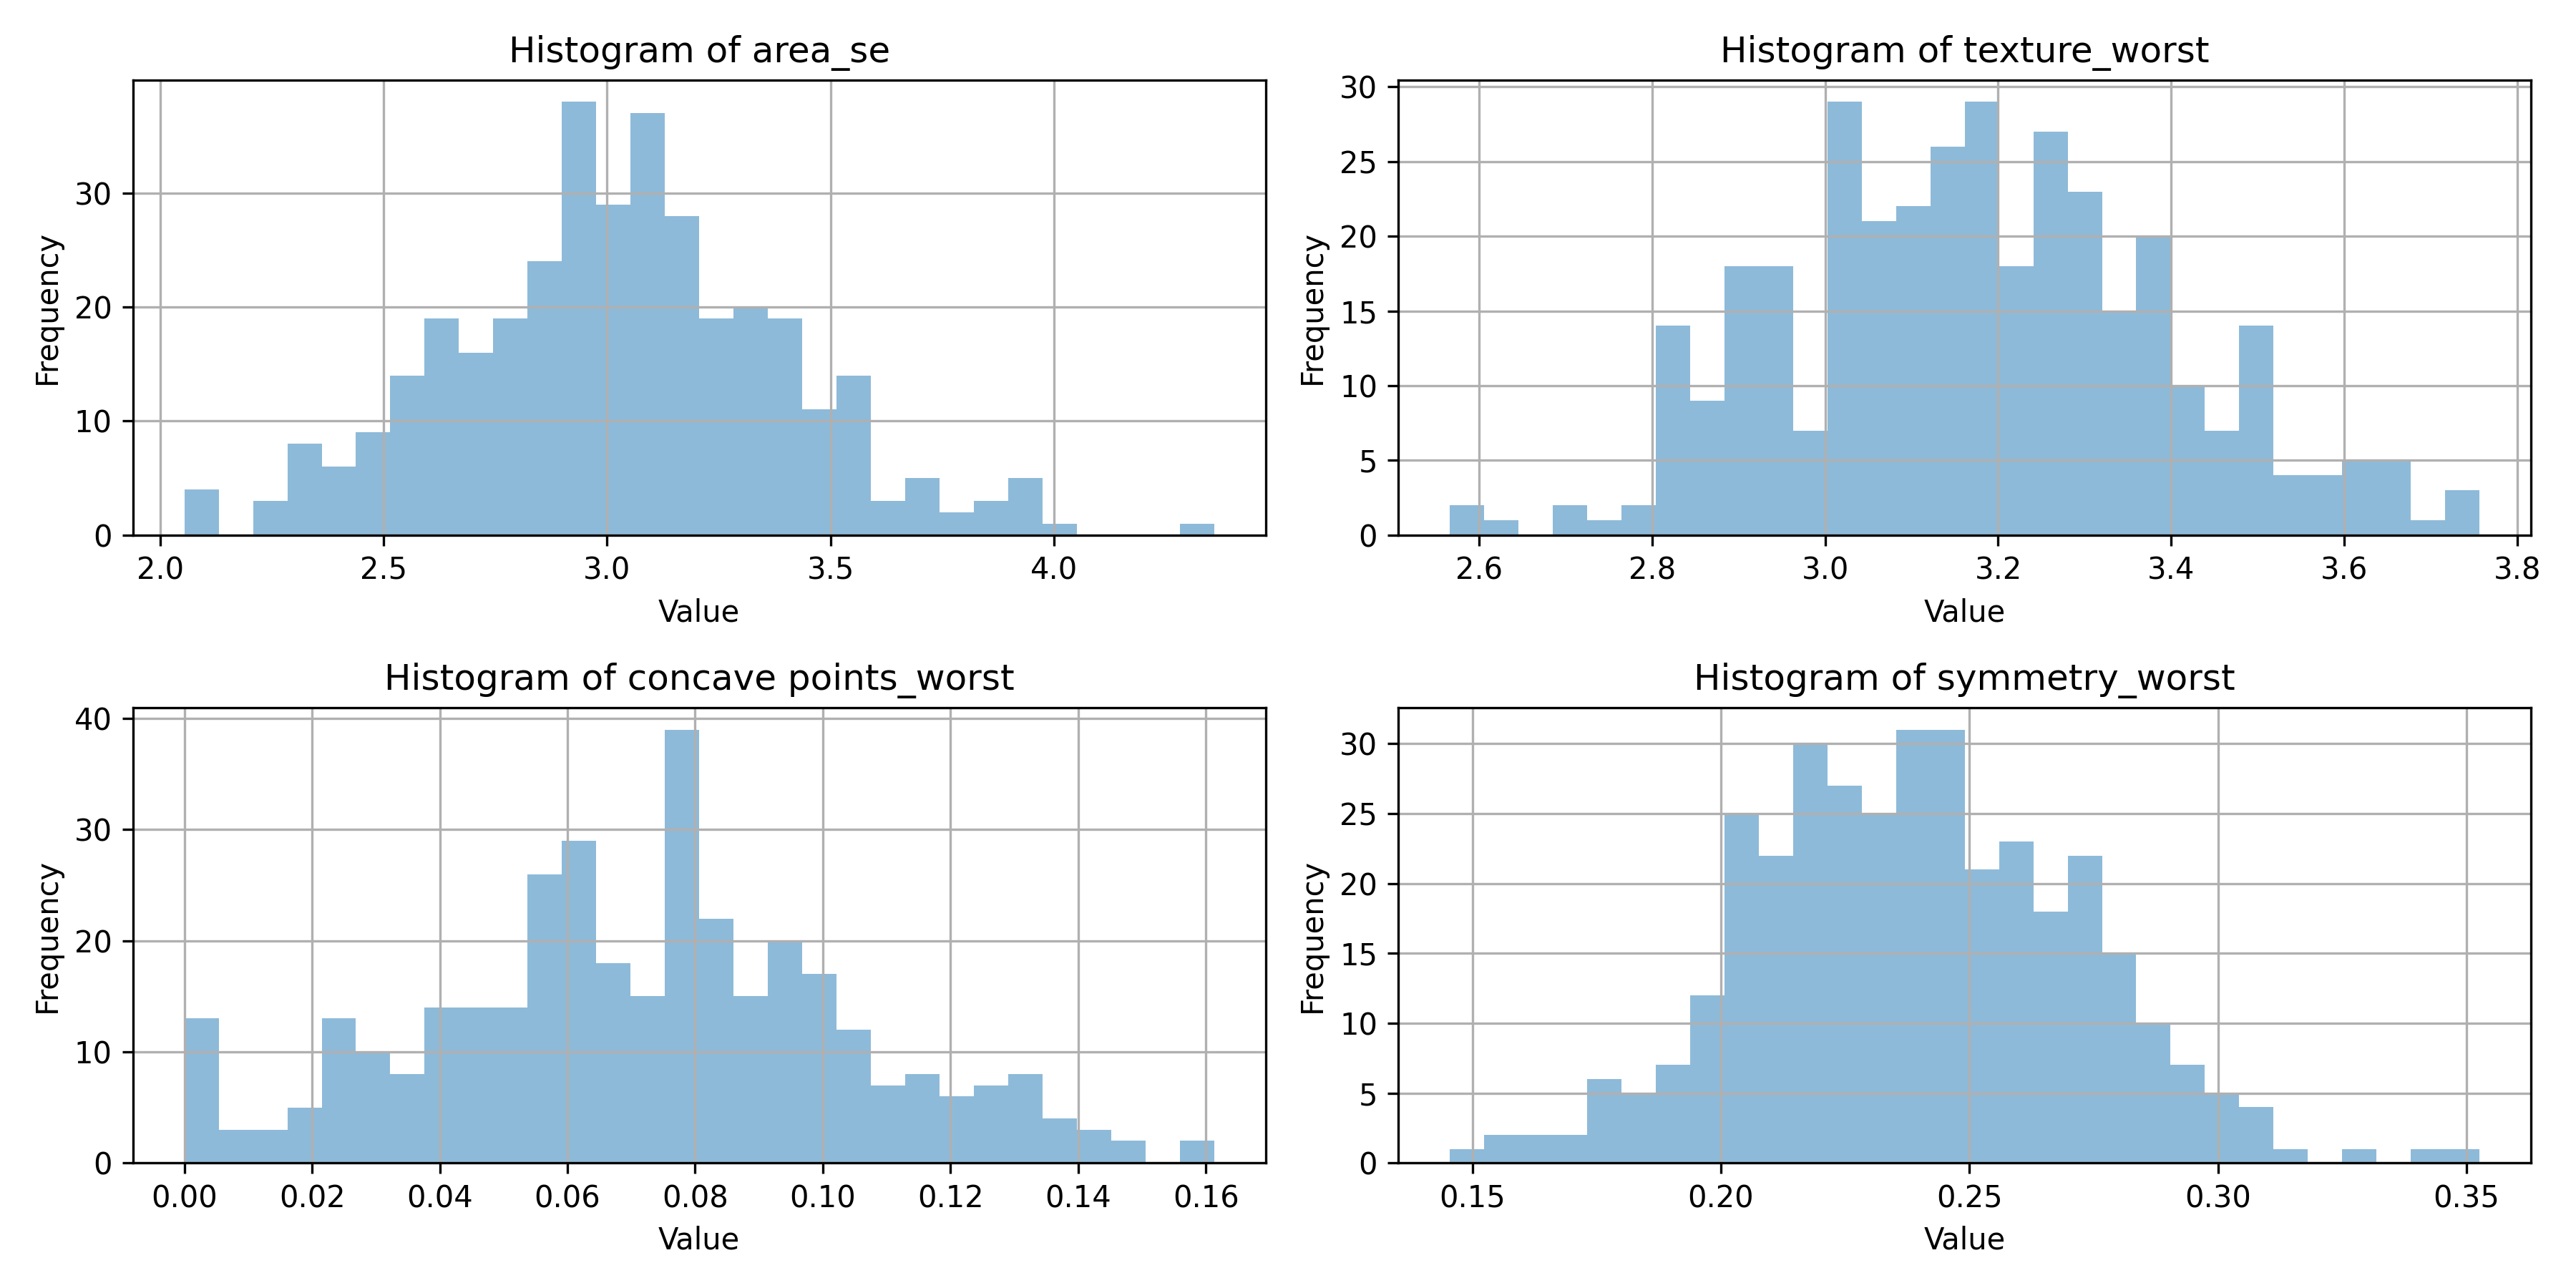
\includegraphics[width=0.9\linewidth]{../results/breast_cancer_normal_distributions.png}
    \caption{Histograms of normal distributions that pass the normality test(corresponding to table \ref{tab:normality_brca})}
    \label{fig:normal_histograms_brca}
\end{figure}

Hence, we will take these four variables as valid normally distributed features as one of the inputs for the iClusterVB method.


We also did Poisson testing on the data, and we found that most variables are not Poisson distributed, 
only one variable \textit{texture\_se} is Poisson distributed.

\begin{table}[!h]
    \centering
    \caption{Chi-square test for all variables in the breast cancer dataset}
    \label{tab:chi_square_brca}
    \begin{tabular}{cccc}
    \toprule
    \textbf{index} & \textbf{Variable} & \textbf{Chi2 Statistic} & \textbf{Poisson-p-value} \\
    \midrule
    3 & texture\_mean & 25.2086 & 0.0000 \\
    4 & perimeter\_mean & 334.8591 & 0.0000 \\
    5 & area\_mean & 232.2412 & 0.0000 \\
    13 & texture\_se & 1.5309 & 0.2160 \\
    14 & perimeter\_se & 63.7165 & 0.0000 \\
    15 & area\_se & 108.8869 & 0.0000 \\
    22 & radius\_worst & 235.0098 & 0.0000 \\
    23 & texture\_worst & 137.9469 & 0.0000 \\
    24 & perimeter\_worst & 353.2600 & 0.0000 \\
    25 & area\_worst & 354.8223 & 0.0000 \\
    \bottomrule
    \end{tabular}
\end{table}

Other variables that are not shown in the table are not suitable for the Poission test, and we assumed they are not Poisson distributed.

To multinomial(bernoulli) test, we found that all variables are not interget-valued, hence they are not suitable for multinomial test.
Therefore, we will not take multinomial test in this case.


\begin{table}[!h]
    \centering
    \caption{Variables Selected for iClusterVB Analysis}
    \label{tab:variables_iclustervb}
    \begin{tabular}{ll}
    \toprule
    \textbf{Variable Type} & \textbf{Selected Variables} \\
    \midrule
    Gaussian (Normal) & area\_se, texture\_worst, concave points\_worst, symmetry\_worst \\
    Poisson & texture\_se \\
    \bottomrule
    \end{tabular}
\end{table}

Table~\ref{tab:variables_iclustervb} lists the variables selected for the iClusterVB analysis. 
The Gaussian variables were chosen based on their normality test results, while the Poisson variable was selected 
based on the Poisson test. These variables serve as inputs for the iClusterVB method, representing distinct data views 
to capture meaningful patterns and relationships in the dataset.


\subsection{iClusterVB Results}

\subsection*{Clustering Summary on Breast Cancer Subset}

The clustering algorithm was applied to a real subset of the breast cancer dataset, yielding the following results:

\begin{table}[!h]
    \centering
    \caption{Clustering Summary for Breast Cancer Subset}
    \label{tab:brca_clustering_summary}
    \begin{tabular}{ll}
    \toprule
    \textbf{Metric} & \textbf{Result} \\
    \midrule
    Total number of individuals & 357 \\
    Maximum number of clusters (user input) & 6 \\
    Number of clusters determined & 6 \\
    \midrule
    Variables selected (posterior inclusion probability > 0.5) & \\
    \quad View 1 - Gaussian & 2 out of 4 \\
    \quad View 2 - Poisson & 2 out of 2 \\
    \bottomrule
\end{tabular}
    
    \vspace{1em}

\begin{tabular}{cccccc}
    \multicolumn{6}{c}{\textbf{Cluster Membership Distribution}} \\
    \toprule
    Cluster 1 & Cluster 2 & Cluster 3 & Cluster 4 & Cluster 5 & Cluster 6 \\
    \midrule
    57 & 55 & 80 & 46 & 98 & 21 \\
    \bottomrule
    \end{tabular}
\end{table}

Table~\ref{tab:brca_clustering_summary} presents the clustering summary for a subset of the breast cancer dataset. 
The algorithm successfully identified 6 clusters from 357 individuals, matching the user-specified maximum number of clusters. 
Cluster sizes ranged from 21 to 98. Variable selection results show that 2 out of 4 Gaussian variables and all 2 Poisson variables were selected based on a posterior inclusion probability threshold of 0.5, 
indicating their importance in distinguishing clusters across the two views.

Figure~\ref{fig:breast_cancer_heatmap} shows the clustering heatmaps for the breast cancer dataset based on two data views: 
(A) Gaussian and (B) Poisson. Each column corresponds to an individual, and rows represent variables.
 The color bars at the top denote the cluster membership of each individual. In both views, clear block patterns are observed,
  indicating distinct variable activity across different clusters. This separation suggests that the clustering algorithm effectively 
  identified subgroups with different underlying characteristics in both Gaussian and Poisson features.

\begin{figure}
    \centering
    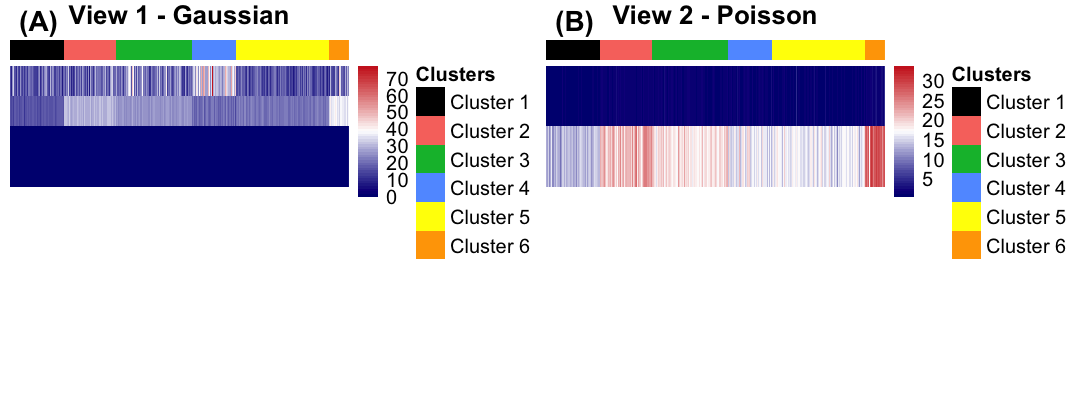
\includegraphics[width=0.9\linewidth]{../results/hamp_real_data.png}
    \caption{Heatmap of the clustering results on breast cancer data}
    \label{fig:breast_cancer_heatmap}
\end{figure}